\documentclass{sigchi}

% Use this command to override the default ACM copyright statement
% (e.g. for preprints).  Consult the conference website for the
% camera-ready copyright statement.


%% EXAMPLE BEGIN -- HOW TO OVERRIDE THE DEFAULT COPYRIGHT STRIP -- (July 22, 2013 - Paul Baumann)
% \toappear{Permission to make digital or hard copies of all or part of this work for personal or classroom use is      granted without fee provided that copies are not made or distributed for profit or commercial advantage and that copies bear this notice and the full citation on the first page. Copyrights for components of this work owned by others than ACM must be honored. Abstracting with credit is permitted. To copy otherwise, or republish, to post on servers or to redistribute to lists, requires prior specific permission and/or a fee. Request permissions from permissions@acm.org. \\
% {\emph{CHI'14}}, April 26--May 1, 2014, Toronto, Canada. \\
% Copyright \copyright~2014 ACM ISBN/14/04...\$15.00. \\
% DOI string from ACM form confirmation}
%% EXAMPLE END -- HOW TO OVERRIDE THE DEFAULT COPYRIGHT STRIP -- (July 22, 2013 - Paul Baumann)


% Arabic page numbers for submission.  Remove this line to eliminate
% page numbers for the camera ready copy 

%\pagenumbering{arabic}

% Load basic packages
\usepackage{balance}  % to better equalize the last page
\usepackage{graphics} % for EPS, load graphicx instead 
%\usepackage[T1]{fontenc}
\usepackage{txfonts}
\usepackage{times}    % comment if you want LaTeX's default font
\usepackage[pdftex]{hyperref}
% \usepackage{url}      % llt: nicely formatted URLs
\usepackage{color}
\usepackage{textcomp}
\usepackage{booktabs}
\usepackage{ccicons}
\usepackage{todonotes}
% \usepackage{natbib}
\usepackage{array}
\usepackage{tikz}

% llt: Define a global style for URLs, rather that the default one
\makeatletter
\def\url@leostyle{%
  \@ifundefined{selectfont}{\def\UrlFont{\sf}}{\def\UrlFont{\small\bf\ttfamily}}}
\makeatother
\urlstyle{leo}

% To make various LaTeX processors do the right thing with page size.
\def\pprw{8.5in}
\def\pprh{11in}
\special{papersize=\pprw,\pprh}
\setlength{\paperwidth}{\pprw}
\setlength{\paperheight}{\pprh}
\setlength{\pdfpagewidth}{\pprw}
\setlength{\pdfpageheight}{\pprh}

% Make sure hyperref comes last of your loaded packages, to give it a
% fighting chance of not being over-written, since its job is to
% redefine many LaTeX commands.
\definecolor{linkColor}{RGB}{6,125,233}
\hypersetup{%
  pdftitle={SIGCHI Conference Proceedings Format},
  pdfauthor={LaTeX},
  pdfkeywords={SIGCHI, proceedings, archival format},
  bookmarksnumbered,
  pdfstartview={FitH},
  colorlinks,
  citecolor=black,
  filecolor=black,
  linkcolor=black,
  urlcolor=linkColor,
  breaklinks=true,
}

% create a shortcut to typeset table headings
% \newcommand\tabhead[1]{\small\textbf{#1}}

% End of preamble. Here it comes the document.
\begin{document}

\title{The Quantified Patient in the Doctor's Office: Challenges in Designing for Clinical Decision-Making Settings}

\numberofauthors{3}
\author{%
  \alignauthor{1st Author Name\\
    \affaddr{Affiliation}\\
    \affaddr{City, Country}\\
    \email{e-mail address}}\\
  \alignauthor{2nd Author Name\\
    \affaddr{Affiliation}\\
    \affaddr{City, Country}\\
    \email{e-mail address}}\\
  \alignauthor{3rd Author Name\\
    \affaddr{Affiliation}\\
    \affaddr{City, Country}\\
    \email{e-mail address}}\\
}

\maketitle

\begin{abstract}
While the \emph{Quantified Self} movement has largely centred around the individual’s own use of his or her data, the same kinds of patient-captured information about their well-being could, in theory, facilitate more accurate and effective medical diagnosis and treatment.  In practice, however, introducing such data during in a way that they can be used effectively and without additional risk during patient visits and hospital episodes creates significant challenges, that we believe, HCI research can help.  In this paper, we seek to understand the primary bottlenecks to the use of QS data during patient visits in both primary and secondar (specialist) care through a literature survey and group 

\end{abstract}

\keywords{Quantified Self; mHealth; Clinical Decision-Making}

\category{H.5.m.}{Information Interfaces and Presentation
  (e.g. HCI)}{Miscellaneous} \category{See
  \url{http://acm.org/about/class/1998/} for the full list of ACM
  classifiers. This section is required.}{}{}

\section{Introduction}

Empowering patients ``take charge'' of their health is an idea frequently championed by politicians~\cite{brown, obama}, technologists~\cite{ihealth}, journalists~\cite{goetz} and healthcare experts alike~\cite{swan2012health}.  Yet, despite countless government and industry-led initiatives across Europe, the UK, and North America, to inspire this ``patient-led healthcare revolution'', it has yet to happen.  

One area, however, where individuals have been taking the lead in trying to understand their own health, is the \emph{Quantified Self} movement \cite{}, primarily comprised of hobbyists and non-health experts who use technological tools to meticulously record and interrogate the minutiae of their physical and mental states over time.   As the population of those interested in self-tracking grew and attracted mainstream interest, the industry has swiftly responded to the expanding demand for self-tracking tools and technologies with a now enormous collection of wearable and embeddable sensors.  These technologies now enable people to record and keep track of aspects of their health with less effort and better fidelity than ever previously, and will continue to improve such as by being less invasive, more comfortable, and more accurate.

While the direct application of such sensors to understanding patients' particular symptoms, situations and lifestyles in the healthcare context would seem straightforward, most physicians today avoid or outright reject the use of self-logged QS data. Even when this information is provided by patients and is reference, it is still rarely, if ever, used for differential diagnosis.  

What are the barriers to the use of self-logged QS data in critical clinical decision making settings?  This is a delicate question to approach for several reasons; first, during the a course of a single patient visit, there may be many kinds of decisions made by a plurality of medical professionals in different roles, in similarly diverse settings.   Paramedics in an ambulance, triage nurses within an emergency room, specialists in a acute care unit or hospital wards, to general practitioners (GPs) in their surgeries, all make decisions regarding a patient under very distinct situational and informational constraints~\cite{croskerry}. Second, even if focus is centred around a single setting, by a single class of medical professionals, such as GP surgeries, there may be significant disparities in the ways different GPs do things; for example, the degree to which GPs use electronic medical records (EMRs)~\cite{hunt} to organise patient data, prescribe particular tests or treatments~\cite{}, or the mechanism and method that they use to maintain good patient relationships~\cite{} can be highly inconsistent. Finally, clinical decision making is a field that is not only long established, but one of the most specialised occupations in the modern workforce; therefore, understanding the effects of the introduction of any new information into such a setting requires an in-depth understanding of the processes, training and tradition.

For our investigation, we focused on two different roles: primary care physicians on the ``frontline'' of the medical service, and secondary care specialists who work in hospitals in specialised units.  In our investigation, we sought to understand the fundamental nature of the barriers to adoption of broadly-classed 'self-logged' patient data, particularly of the most common types facilitated by the many kinds of consumer health monitoring tools becoming available.  That is, we wished to identify whether reasons that such self-logged data were still, so often, deemed useless by clinical professionals, included \emph{what} was captured, how it was captured, the ways in which it was represented or made available during a patient consultation, or  due to other, yet unidentified problems derived from looking at or processes required to derive insight from it.  From this, we wished to extrapolate how such problems might help be shaping and solved through HCI research, such as by re-thinking tools people used to monitor themselves, the kinds of data they captured, or the ways that physicians and medical professionals might access and use it, towards the visions of eHealth and mHealth set out so often in the popular press (e.g. ~\cite{goetz, thingy, thingy}).

\section{Overview of Approach}

We began with an initial set of broad dimensions (Figure \ref{fig:qs}) chosen to represent the potentially many kinds of reasons that self-logged, QS data remains far from fulfilling its potential in clinical practice.

\begin{figure}[tbpb]
\begin{enumerate}
    \item \emph{Data subject}: Lack of relevance or utility of \emph{what} is captured
    \item \emph{Sampling method}: Problems with \emph{how} and \emph{when} information is captured
    \item \emph{Accuracy}: Lack of trust in accuracy of instruments or capture method
    \item \emph{Access}: Problems with physician \emph{access} to the data
    \item \emph{Patient communication}: Interference with patient clinician communication
    \item \emph{Workflow}: Interference or exclusion from diagnostic workflow
    \item \emph{Biases}: Danger of cognitive biases introduced by data?
    \item \emph{Other}: External factors? (\emph{data handling}, \emph{legal}, \emph{billing} etc)
\end{enumerate}
\caption{Initial dimensions for categorising barriers to clinical use of self-logged/QS data.}
\label{fig:qs}
\end{figure}

Since these dimensions encompassed a broad set of possible factors, including data-oriented problems (such as pertaining to subject, quality and sampling), situational constraints, and practice constraints, we wished to understand which, if any, of these dimensions had support from previous studies.  This lead us a broad survey of medical literature, which we describe in the next section.  

Then, to investigate whether we could gather primary evidence towards the importance of any of these dimensions, we followed with a role-play study in which practicing GPs and specialists were presented with patient illness scripts, based on real cases, in which patients brought various QS data with them while in the process of presenting their complaint.  We asked GPs and specialists to come up with their own diagnosis, following a think-aloud protocol.  We then transcribed, annotated and derived codes from each session to identify reasons the QS data were or were not consulted, and ways that the presence of the QS data influenced the diagnostic process.  From these codes, we derived a set of themes, which we then used to compare our findings to previous findings in the literature.  Finally, we discuss the limitations of our study and future work.

% To undestand this method we conducted a two phase invesitgation. Fi


% This paper presents a collective summary of our initial investigation in 

%Second, medical decision-making is making  we wish to approach this question carefully, considering What are doctors, nurses, specialists and medical professionals' views on the QS movement and self-logged data?  Is it a problem of what is being captured, how it is being captured, how it is represented, or presented?  In this paper, we summarise an initial exploration of these questions comprised of two stages: first, a literature survey pre-study, which informed the design of a set of role-playing probes with clinical specialists.


\section{Background} 

We contextualise our investigation against two closely related fields: the first, \emph{evidence based medicine} sought to expand the use of empirical methods (such as used in epidemiology) for evaluating and improving the effectiveness of decisions such as those affecting treatment choices.  The second, \emph{clinical decision making} examines the cognitive, interactional and situational processes which influence how practitioners arrive at decisions, under the practical constraints necessary for conducting their practices.  In this section, we first introduce at a high level, common visions of how technology-enabled, patient data-driven healthcare might be realised in the future.  We then discuss evidence-based medicine and the role of clinical decision making literature to our investigation.

\subsection{Visions for Data-driven eHealth / mHealth}
Notions of ``big data'' and ``data driven healthcare'' have inspired many visions  for more data-informed healthcare internationally. In the popular press, Thomas Goetz's \emph{The Decision Tree} outlined a vision in which every person will be DNA-tested at birth, and tracked with sensors throughout their lives; the resulting piles of data would be used to classify and compute (through statistical measures) optimal treatments and actions. Policy makers have set out national agendas towards such a goal; the UK's Personalised Health and Care 2020 framework set out a vision in which health and well-being data, sensed from wearable and environmental sensors, would seamlessly integrate with patient health records by 2018~\cite{Personalised2014}.  The framework proposes that these data would ``fill in the gaps'' between visits with their GP or specialist, enabling clinicians to more effectively perform personalised differential diagnosis at point of care.  It is anticipated that the introduction of such technologies will simultaneously improve outcomes substantially and drive down costs.  Other visions include use in preventative medicine, to enable early onset detection of chronic conditions, thereby potentially reversing the course of conditions before they set in~\cite{Swan2009}.  Exploratory data mining of sensed data is also likely to radically improve our understanding of both prominent and rare medical conditions, by revealing relationships among genetic, lifestyle, and environmental factors that might contribute to patients' symptoms.  Initial enthusiasm for this vision is also evident in the US, with the US Food and Drug Administration's approval of  consumer tracking devices for clinical trials, citing the importance of quantifiable analysis of physical activity to physiological monitoring~\cite{U.S.FoodandDrugAdministration2014}.

% quantified self vs self tracking vs lifelog vs prescribed sensors vs personal health records

% dont have much basis of saying this

Responding to this interest, the race to attract end-user consumers to better and more accurate physiological sensors has taken off past 8 years. New, freshly funded companies such as Withings, FitBit and Jawbone, have been joined veteran sport performance monitoring device makers such as Garmin, while established brands for sport to consumer electronics, such Nike and Sony have joined the fray to each develop attractive wearable personal tracking devices.  While still a minority, several, namely at the time of writing iHealth and Withings, have had several of their consumer-level sensors certified for clinical use, as under the US FDA Class-1 and 2 medical device classification scheme. 

%\section{Barriers to Adoption}

% Yet despite this industry, political and tech-driven enthusiasm for use of self-logged QS data, clinical uptake has been slow.  For example, even with Apple's partnership with US healthcare providers around the targeted of their HealthKit framework have focused primarily on its use in telemonitoring for randomised controlled trials (RCT) rather than for differential diagnosis.  But even here, problems have been met with some partners pulling out, citing insufficient interest by both patients and physicians~\cite{}.  

% An informal survey by VentureBeat found that clinicians were largely ''simply not interested in FitBit data'', assigning blame on several factors~\cite{venturebeat}. The first was time; doctors cited simply not having the time to look at data brought in by patients.  The second pertained ot access; electronic medical records simply did not admit or integrate patient-supplied data.  Third were concerns about data quality, e.g. that devices available today were simply not yet accurate enough for clinical use.  Finally, doctors expressed legal concerns around use of the data; citing the potential to be held liable for data captured by wearable health sensors.

\subsection{Evidence Based Medicine: Clinical Decision-Making with Data under Uncertainty} 

The term \emph{evidence-based medicine} refers to the use of epidemiological methods in both patient-level decision making and formulation of population-level clinical care guidelines.  In the first use of the term, David M. Eddy pointed out that, while outcome analysis may make it seem that there is a clear path towards achieving more accurate, or at least consistent, diagnoses, things are never that simple in practice~\cite{eddy1990challenge}:

\begin{quote}
  Decisions might be variable but they are not whimsical or flippant. The variability occurs because physicians must make decisions about phenomenally complex problems, under very difficult circumstances, with very little support. They are in the impossible position of not knowing the outcomes of different actions, but having to act anyway.
\end{quote}

Eddy, thus, argues that, that due to the nature of the complexities of assessing individual patients' conditions under the constraints in place, care targets and practice recommendations alone will not achieve better health outcome.  Instead, working under extreme uncertainty is a necessity and should be embraced with the acknolwedgement of the effects of various decision-making constraints and biases that are known to exist.

\subsection{Clinical Decision-Making} 

% TODO TODO 
Clinical decision-making biases have long been studied in the medical community.  
Modern texts for nursing and clinical evaluation have formalised the diagnostic process of determining a patient's disease or condition based on available evidence, including presenting symptoms as a technique known as \emph{differential diagnosis}~\cite{thompson2002clinical}.  This is usually described as some variation of the following procedure: First, the physician gathers all information available about the patient, creating a list of the patient's symptoms.  Then, she or he lists all possible candidate conditions for the symptoms, which is then prioritised with most the urgently dangerous possible causes first.  Finally, possible causes are ruled out or treated systematically.  

\subsection{Cognitive Dispositions to Respond}

Recent research has revealed that clinical decision-making is often strongly influenced by cognitive bias, leading to preventable adverse events, worsened patient outcomes, and higher mortality.  Croskerry et al. characterised a ~\citep{Croskerry2013}. \citet{Graber2002} states that cognitive bias is a major cause of preventable diagnostic error, but is extremely challenging to study and reduce. This complements earlier discoveries by \citet{Kahneman1982}, in which people tend to use biases when making decisions under uncertainty, occasionally leading to severe errors. Many forms of cognitive bias have been identified -- Wikipedia lists over 350\footnote{Wikipedia -- List of cognitive biases -- \url{http://en.wikipedia.org/wiki/List_of_cognitive_biases} [Accessed 4th Sep 2014]} -- however, the consequences of biases in clinical decision making remain largely unexplored \citep{Croskerry2013}. It is thus unknown how the provision of patient data may affect bias in clinical decisions.

% research questions
% By conducting a literature review of research in cognitive bias over the last 50 years, this dissertation presents a list of 11 cognitive biases which may affect clinical decisions made when patient data is used. From this, it has been identified that supplementing patient data may introduce further bias due to methods clinicians use to interpret patient data. Furthermore, it has been found that these biases usually have a more significant effect when decisions are made in acute scenarios, such as emergency rooms, where decisions must be made quickly with limited resources.

% definitions
%For the purpose of this paper, decisions which involve patient data are called \textit{evidence-based clinical decisions}. The term \textit{patient data} refers specifically to personal information which is collected by mobile apps and consumer devices, such as the number of steps taken, video lifelogs, location history and status updates on social networks. Patient data is subsequently \textit{interpreted} by clinicians, which refers to the observation, analysis and sense-making of data.


% stuff from pete's masters thesis

% a little bit about all the potential ways QS could help

% \cite{Swan2009} has called for use of this data as a means to supplement healthcare, which would increase ``information flow, transparency, customization, collaboration and patient choice and responsibility taking, as well as quantitative, predictive and preventive aspects.''. The use of self-tracking data in healthcare is not new. The health diary has been popular since the 1950's as a data collection method \cite{Richardson1994}.  \cite{Richardson1994} note that particular types of data that are recorded include pain, fatigue, medication use and dietary intake. This shares overlap with health and wellbeing data, suggesting there are existing use cases where health and wellbeing data could be supplemented. \cite{OLoughlin2013} has demonstrated the use of lifelogging for the purpose of increasing diet awareness. However, \cite{Swan2009} has discussed that there is currently little adoption, perhaps due to the barriers of technology in clinical environments.


\section{Pre-study: Literature Review} 

We anticipated that the slow uptake of the use of self-logged QS could potentially be attributed to a large number of factors, and thus decided it prudent to first do a survey of medical, quantified-self and HCI literature.  Our objective  was to establish a theoretical framework from which we could then identify areas that could require further investigation, as well as opportunities where research in HCI could potentially help.  

\subsection{Literature Review: Method}

We started with a set of search terms broad enough to encompass studies of clinical practice where patient-logged data (both paper-based and digital, manual and automatic) were introduced into a clinical setting.  To do this we searched PubMed, Google Scholar and the ACM DL for keywords ``patient diaries'', ``care diaries'', ``wellbeing diaries'', ``self-report diaries'', ``quantified-self'', ``smartphone apps'', and ``wearable sensors''.

Since we wanted to focus on the usage of data by medical experts, we excluded studies about use by patients themselves, such as for feedback, reflection, goal setting and self monitoring, including behaviour-change studies and studies of motivation to self-diaries, which were prevalent from the HCI community.   Focusing only on existing practice, we omitted papers describing new interfaces and systems that have not had substantial adoption.  We also excluded papers discussing the capture side of health diarising and life-logging by patients, except where aspects of capture affected its later use.  We were careful to include papers that discussed any issues relating to the use of patient data in clinical setting, including those that discussed human factors issues specifically, to more broadly  theatres and emergency rooms.

After finding a small set of results, we then broadened our search to include studies that discussed the use of patient data in medical decision-making, including both patient-supplied and clinical data held by providers themselves.  We included ``telemonitoring'', and ``electronic patient records''.  This  hoped to find a broad range of factors spanning human-factors issues to social, cultural, institutional, situational, among others.

For each paper, we identified problem(s) in the clinical use of data, which were first added to a spreadsheet and linked to their original source.  After examining each of the papers, 2 researchers organised the list into themes, attempting to merge all problems with the same underlying cause, while keeping those that did not overlap distinct.  During this process, we identified a set of themes related specifically to cognitive biases, which we analysed and report separately below.

Excluded papers relating to self-recorded data which patients were asked to record by their physicians, such as papers containing the words "telemonitoring" or "telemedicine". Literature reviews were excluded. 

%Papers discussing the accuracy or reliability of self-management did not disc

\subsection{Literature Review: Results}

From an initial set of 2340 results, we identified 429 papers that actually contained at least one of the search terms among keywords and the abstract. From here, we identified $XX$ relevant papers according to the criteria defined above.  From this we derived the $CC$ themes visible in \ref{fig:themes}, omitting themes pertaining to cognitive dispositions to respond which we discuss next.

% @@@@@@@@@@@@@@@@@@@@@@@@@
%
% initially focused on "use of self-recorded data by clinicians", but there is little literature on this. we then broke down the literature review into individual factors:
% * reliability of self-recorded data
% * use of IT by clinicians (e.g. EMR)
% * cognitive factors when clinicians interpret information
%
% @@@@@@@@@@@@@@@@@@@@@@@@@

\def \w {$\bullet$}

\subsubsection{High-level Themes}

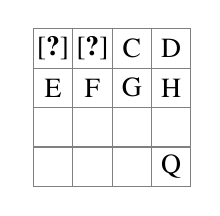
\begin{tikzpicture}
\draw[step=0.5cm,color=gray] (-1,-1) grid (1,1);
\node at (-0.75,+0.75) {\cite{chung_more_2015}};
\node at (-0.25,+0.75) {\cite{ancker_invisible_2015}};
\node at (+0.25,+0.75) {C};
\node at (+0.75,+0.75) {D};
\node at (-0.75,+0.25) {E};
\node at (-0.25,+0.25) {F};
\node at (+0.25,+0.25) {G};
\node at (+0.75,+0.25) {H};
% ...
\node at (+0.75,-0.75) {Q};
\end{tikzpicture}

\begin{tikzpicture}
\draw[step=0.5cm,color=gray] (-4,-1) grid (22,18);
\node at (-4,-1) {\textbf{Factor}}
\node at (0,-1) {\cite{chung_more_2015}}
\node at (1,-1) {\cite{ancker_invisible_2015}}
\node at (2,-1) {\cite{becker_mhealth_2014}}
\node at (3,-1) {\cite{sullivan_guess_2014}}
\node at (4,-1) {\cite{almalki_use_2015}}
\node at (5,-1) {\cite{patel_probing_2012}}
\node at (6,-1) {\cite{Swan2009}}
\node at (7,-1) {\cite{millar_shared_2004}}
\node at (8,-1) {\cite{ancker_you_2015}}

% use of IT by clinicians
\node at (9,-1) {\cite{alsos_mobile_2012}}
\node at (10,-1) {\cite{frankel_effects_2005}}
\node at (11,-1) {\cite{zeldes_information_2011}}
\node at (12,-1) {\cite{chen_unpacking_2011}}
\node at (13,-1) {\cite{patterson_human_2004}}
\node at (14,-1) {\cite{schoenberg_weaving_2000}}
\node at (15,-1) {\cite{vikkelso_subtle_2005}}
\node at (16,-1) {\cite{hughes_2.0_2008}}

% reliability/accuracy of self-recorded data
\node at (17,-1) {\cite{demonceau_contribution_2015}}
\node at (18,-1) {\cite{tsoukalas_data_2015}}
\node at (19,-1) {\cite{frier_hypoglycaemia_2015}}
\node at (20,-1) {\cite{khariwala_self-reported_2015}}
\node at (21,-1) {\cite{dontje_measuring_2015} }}

\node[fill=black] at (0,0) {}

\end{tikzpicture}


\begin{table*}
    \setlength\extrarowheight{0.1cm}
    \setlength\tabcolsep{0pt}
    \centering
    \begin{tabular}{>{\raggedright}p{4.3cm} |
        | >{\centering}p{0.6cm} | >{\centering}p{0.6cm} | >{\centering}p{0.6cm} | >{\centering}p{0.6cm} | >{\centering}p{0.6cm} | >{\centering}p{0.6cm} | >{\centering}p{0.6cm} | >{\centering}p{0.6cm} | >{\centering}p{0.6cm} 
        | >{\centering}p{0.6cm} >{\centering}p{0.6cm} >{\centering}p{0.6cm} >{\centering}p{0.6cm} >{\centering}p{0.6cm} >{\centering}p{0.6cm} >{\centering}p{0.6cm} >{\centering}p{0.6cm} 
        | >{\centering}p{0.6cm} >{\centering}p{0.6cm} >{\centering}p{0.6cm} >{\centering}p{0.6cm} >{\centering}p{0.6cm}}
        
    \toprule
    & \multicolumn{9}{>{\centering}p{5.4cm}|}{Clinical use of self-recorded data}
    & \multicolumn{8}{>{\centering}p{4.8cm}|}{Clinical use of IT}
    & \multicolumn{5}{>{\centering}p{3.0cm}|}{Reliability of self-recording} \\
    
    \textbf{Factor}
    % use of self-recorded data by clinicians
    & \cite{chung_more_2015}
    & \cite{ancker_invisible_2015}
    & \cite{becker_mhealth_2014}
    & \cite{sullivan_guess_2014}
    & \cite{almalki_use_2015}
    & \cite{patel_probing_2012}
    & \cite{Swan2009}
    & \cite{millar_shared_2004}
    & \cite{ancker_you_2015}
    
    % use of IT by clinicians
    & \cite{alsos_mobile_2012}
    & \cite{frankel_effects_2005}
    & \cite{zeldes_information_2011}
    & \cite{chen_unpacking_2011}
    & \cite{patterson_human_2004}
    & \cite{schoenberg_weaving_2000}
    & \cite{vikkelso_subtle_2005}
    & \cite{hughes_2.0_2008}
    
    % reliability/accuracy of self-recorded data
    & \cite{demonceau_contribution_2015}
    & \cite{tsoukalas_data_2015}
    & \cite{frier_hypoglycaemia_2015}
    & \cite{khariwala_self-reported_2015}
    & \cite{dontje_measuring_2015} } \\
    
        \midrule 
    \textbf{Data capture}} \\
    capture irrelevant/useless things
        &\w &\w &   &   &   &\w &   &   &   &   &   &\w &   &\w &   &   &   &   &   &   &   &  \\
    poor data quality
        &   &   &   &\w &   &\w &   &   &\w &   &   &   &   &\w &   &   &\w &\w &\w &   &   &\w }\\
    data incomplete
        &   &\w &\w &   &   &\w &   &   &\w &   &   &   &   &\w &   &\w &   &   &   &\w &\w &  \\[0.4cm]
        %\midrule
    \textbf{Data access}} \\
    no standard for data representation
        &\w &\w &\w &   &   &   &   &   &   &   &   &   &   &   &   &   &   &   &\w &   &   &  \\
    selective disclosure
        &\w &\w &   &   &   &   &   &\w &   &   &   &   &   &   &   &   &   &   &   &   &\w &  \\
    poor interoperability
        &\w &\w &\w &   &   &   &   &\w &   &\w &   &   &\w &   &\w &   &   &   &\w &   &   &  \\[0.4cm]
        %\midrule
    \textbf{Clinical practice}} \\
    no standard methods for interpretation
        &   &   &   &   &   &   &   &   &   &   &   &   &   &   &   &   &   &   &   &   &\w &\w \\
    no data analysis training
        &\w &   &\w &   &\w &   &\w &   &   &   &   &   &   &\w &   &\w &\w &   &   &   &   &  \\
    takes time away from patient
        &\w &   &   &   &   &   &   &   &\w &\w &\w &   &\w &\w &   &   &   &   &   &   &   &  \\
    threatens professional autonomy
        &   &   &   &   &   &   &   &\w &   &   &   &   &   &   &   &\w &   &   &   &   &   &  \\
    legal issues
        &   &   &\w &\w &   &   &\w &   &   &   &   &   &   &   &   &\w &   &   &   &   &   &  \\[0.4cm]
        %\midrule
    \textbf{Situational constraints}} \\
    time pressure
        &\w &   &   &   &   &   &   &   &   &   &\w &\w &   &\w &   &\w &   &   &   &   &   &  \\
    information overload
        &   &   &\w &\w &   &   &   &   &   &   &   &\w &   &   &   &   &   &   &   &   &   &  \\
    not worth clinician effort
        &\w &   &   &   &   &   &   &   &   &   &   &   &   &   &   &   &   &   &   &   &   &  \\
    
    \bottomrule
    \end{tabular}
    \caption{Major themes}~\label{tab:biases}
\end{table*}


%% party here

% \subsubsection{Cognitive Dispositions to Respond}

% During the first phase, we encountered a substantial body of work pertaining to  situational and psychological factors that influenced the decision-making performance of medical experts in clinical settings.  Croskerry's \emph{Cognitive Dispositions to Respond}~\cite{} 

% We started with MEDLINE, Web of Science, and the ACM DL
% Using the keywords "medical decision-making", "clinical decision-making", "patient-logged data", "quantified self", "data in hospital admission", "GP visit", searches were performed on BMJ, MEDLINE, CINAHL, Google Scholar, Web of Science, Springer, and the ACM DL.  This collectively resulted in 2982 results, many of which
% d
% Temporal constraints
% Situational constraints
% UI/UX constraints 
% Workflow constraints
% Cognitive Biases
% Training/background constraints
% Exclusion criteria:
%   Anything that only involved the patient, including behaviour change studies


%   UK Prime Minister Gordon Brown,  pronounced in 2008 that more effective ``future will be one of patient power, patients engaged and taking control over their own health and healthcare.” – Gordon Brown, U.K. Prime Minister



% functional fixedness - doctors _did_ use the data for other 
% confirmation bias - using particular data sources to support a particular hypothesis
% framing
% functional fixedness

\subsubsection{Implications from bias}


\begin{table*}
    \centering
    \begin{tabular}{>{\raggedright}p{1.9cm} p{7.5cm} p{5.8cm} p{1.4cm}}
    \toprule
    {\small\textbf{Factor}}
    & {\small \textbf{Explanation}}
    & {\small \textbf{Implications for use of patient-provided data}}
    & {\small \textbf{Literature sources}} \\
    \midrule
    
    Contextualisation % Problems relating to how a clinians puts a problem in context - their previous experience, framing, approach to risk
    &   \begin{itemize} \parskip0pt \vspace{-2.4mm}
            \item \textit{Priming} - exposure to one piece of information influences how another piece of information is perceived.
            \item \textit{Availability} - the disposition to judge things as being more likely or frequently occurring if they readily come to mind, such as recent information. % e.g. recent experience  with hearing about a disease may inflate the likelihood of its being diagnosed
            \item \textit{Framing} - the way in which a problem is presented affects the outcome of a task.
            \item \textit{Risk taking} - clinicians switch between risk aversion and risk taking depending on whether the problem is expressed in terms of the possibility the patient might die or live.
        \end{itemize}
    & Clinicians see many patients, and their prior decisions or interpretations made with patient-logged data may change how they use new data. Therefore, some pieces of information may become disproportionately relied upon based on inaccurate estimates of frequencies. Further, the patient's approach to providing their data (e.g., why they recorded it) may contribute to a clinicians framing of the problem. This has strong implications for how data may be presented by a patient, and the order data are presented in.
    %The order in which self-logged data are presented, and during a presentation of complaints to a physician. Earlier decisions or interpretations may therefore affect the performance of later decisions or interpretations. which may result in an incorrect diagnoses. 
    %  A clinician may base their diagnoses on the perceived likelihood of a particular disease, which may be influenced by what the clinician has observed previously,
    
    & \cite{Reay2013}, \cite{Kahneman2012}, \cite{Croskerry2002},  \\
    
    Information interpretation %Bias may affect how information is interpreted
    &   \begin{itemize} \parskip0pt \vspace{-2.4mm}
            \item \textit{Illusory patterns} - seemingly meaningful relationships are seen in random data which, despite their statistical insignificant, may be used to influence a decision.
            \item \textit{Representativeness} - when presented with information specific to a patient, other sources of data are neglected (e.g., base rates of a particular disease).
            \item \textit{Anchoring and adjustment} - the tendency to perceptually lock onto prominent features in a patient’s presentation too early in the diagnostic process, and failing to adjust this initial impression in the light of later information. Anchoring has been found to lead to premature decision making with patients being labelled with a diagnosis early in presentation.
            \item \textit{Base rate neglect} - statistical significance of an observation has little influence on its importance in reasoning.
        \end{itemize}
    & Errors made during information processing may may lead to misdiagnoses, rationalising unusual diseases, overutilisation of resources, and contribute to inaccurate estimates of base rates. An observer's ability to appraise the importance of particular pieces information over others may lead a physician to ignore critical pieces of data that were not among those first noticed, such as base rate, the patient's presentation or the patient's medical record.
    & \cite{Whitson2008}, \cite{Kahneman2012}, \cite{Kahneman1978}, \cite{Bar-Hillel1980}, \cite{Croskerry2002}, \cite{Gruber} \\
    
    Metacognition % The cognitive state of the clinician
    &   \begin{itemize} \parskip0pt \vspace{-2.4mm}
            \item \textit{Affect heuristic} - a clinician's emotional state can significantly affect their interpretation of patient data and their decisions
            \item \textit{Confirmation bias} - findings are emphasised based on if they support one's own desires or beliefs
            \item \textit{Selective exposure} - people are less willing to eliminate an original hypothesis, with a person attributing unjustified rationality to that hypothesis based on their pre-existing views.
            \item \textit{Ambiguity effect and outcome bias} - if the probability of favourable outcome is only available for some options, other options tend not be considered, also causing the belief that favourable outcomes are more likely.
            \item \textit{Functional fixedness} - limitations of tools or analysis techniques may lead to a relying on known examples, which may limit insights which may be gained from data
            \item \textit{Appropriation difficulty} - problem solving has been demonstrably less effective when a solution requires atypical use of an object
        \end{itemize}
    & Data interpretations and decisions made using data are ways impacted by emotion and irrational belief in an original hypothesis, despite evidence to the contrary. This may lead to errors and adverse events including incorrect and missed diagnoses. Further, the inability of a clinician to use appropriate data effectively increases the time cost of using data, and limits the capability of a clinician to gain insight from data. In specialist clinical roles, this may lead to only using data in ways that they have been trained in their specialism.
    & \cite{Kahneman2012}, \cite{Finucane1998}, \cite{Nickerson1998}, \cite{Wason1960}, \cite{Croskerry2002}, \cite{Ellsberg1961a}, \cite{Adamson1952}, \cite{German2005} \\
    
    \bottomrule
    \end{tabular}
    \caption{Implications from bias when there are time constraints, constraints on how data may be controlled, or it is not clear how data should be used}~\label{tab:biases}
\end{table*}


\section{Methodology}

May - June 2015

Inspired by methodology from other research

% role-play 
A focus group and two interviews were conducted

Recognise the value of self-logged data

% we derived scenarios from NYT "Think Like a Doctor" 
% how we chose the specific scenarios

\subsection{Recruitment}

\subsection{Analysis}

Two interviews

One focus group

\section{Results}

Participants in the focus group - seven specialists in the US (six male) and three NHS GPs in the UK.

Can we rely on the data?

\subsection{Summary of findings}

\section{Discussion}


\subsection{Implications for design}

\subsection{Limitations}
\susbection{Future Work}

it's not just what the data is, it's who it comes from {your friend, your colleague, your doctor}. is it {a teenager, a female student, a male student, a middle aged man, a middle aged woman}


\section{Conclusions}


% REFERENCES FORMAT
% References must be the same font size as other body text.
\bibliographystyle{SIGCHI-Reference-Format}
\bibliography{wsi-chi-16}

\end{document}

%%% Local Variables:
%%% mode: latex
%%% TeX-master: t
%%% End:
